\documentclass{article}
\usepackage[utf8]{inputenc}
\usepackage{graphicx} 
\graphicspath{ {./images/} }

\title{PS6 Yarberry}
\author{Megan N.Yarberry }
\date{March 3, 2020}

\begin{document}

\maketitle

\section{Introduction}

For my project and thesis topic, I am researching and looking at the donation patterns and one of the major factors. A major factor is how well the football team does, with a correlation to financials. For this assignment, I scrapped several sites for data on financials such as coaching salaries, total athletic department spending along with the number of national championships a program has won. With scraping this data it was pretty clean besides deleting a few rows. For one of the data frames, I went through and renamed a few of the cells for the number of counts. Along with turning the " -- " cells into na so when I went to create a mean it was able to run. Another issue I ran into was converting dollar allocated cells to integers and removing the dollar signs which turned the data from a char to an integer, so I was able to create a visual image of the data.  
\section{Visualization 1}
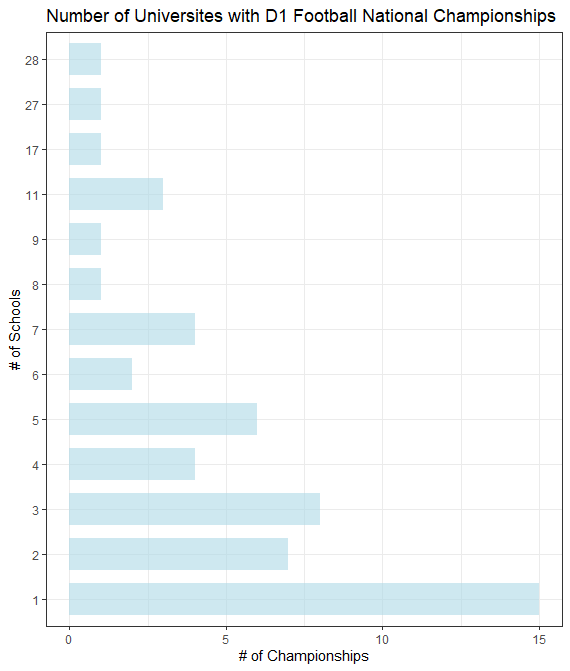
\includegraphics[scale=.75]{PS6a_Yarberry.png}

The first image is a visualized of the number of NCAA National Championships Universities has earned. A visual way of depicting that 15 Football teams having only 1 National Championship, while 3 schools have 11 National Championships and only one University has 27 and 28 titles. I think this helps the gap of which schools have been powerhouses in Football, and that several schools only have one, and how many schools only have like one, two and three national championships. 

\section{Visualization 2}
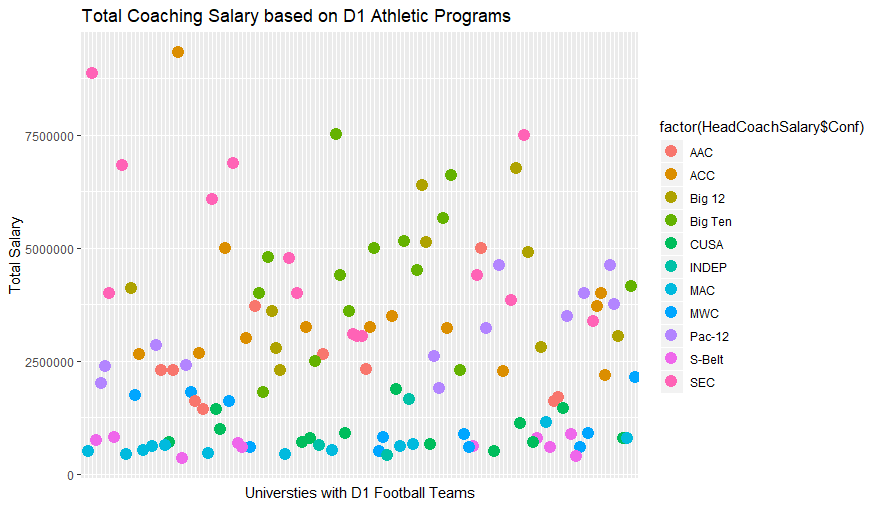
\includegraphics[scale=.75]{PS6b_Yarberry.png}

In the second visualization, I wanted to look at a scatter plot of how much each team was spending on total football coaching expenses, these numbers including the head coach and all the assistance. I decided to remove the names of the Universities and programs because I want to focus more on the conference and if there is a correlation between money spent and being in the same conference and eventually see the correlation between how many National Championship that conference and then the program has. 
\section{Visualization 3}
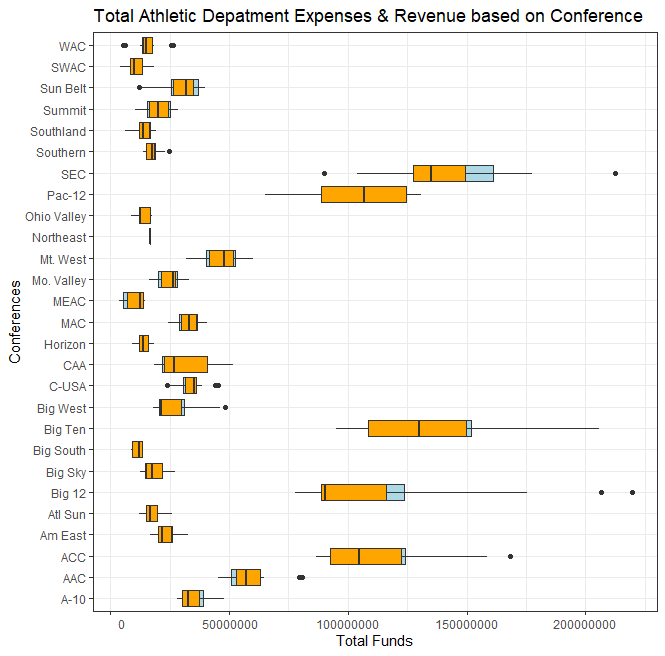
\includegraphics[scale=.75]{PS6c_Yarberry.png}

My third and last visualization is a conference sum of how much each conference is spending, I choose to depict this with a scatter plot so you can see the outliers in each conference along with the median and averages. I overlapped this graph looking at revenue and expenses at the same time. In the orange is the revenue while light blue is the expenses. As you can see from the chart many programs and conferences have a mean average of having a little more revenue than expenses. Meaning programs are generating more revenue then they are spending, not causing a deficit from the season. Very few athletic departments run on surplus for the season and this is interesting to look at and visualize to see exactly what conferences are and also see how large the gap and differences between the top-funded and bottom funded programs are in the same conference. 

\end{document}
